\section{Detecção de ciclos}

\begin{frame}[fragile]{Detecção de ciclos}

    \begin{itemize}
        \item Um ciclo é um caminho de tamanho maior ou igual a três cujos pontos de partida e 
            chegada são iguais

        \item Um grafo que não contém nenhum ciclo é dito acíclico

        \item Uma travessia por profundidade pode ser utilizada para se determinar se um
            componente de um grafo é ou não acíclico

        \item Se, durante a travessia, um dos vizinhos do nó já foi visitado, e este vizinho 
            não é o nó que o antecedeu na busca, então existe um ciclo começando e terminando
            no nó atual, e que passa por este vizinho

        \item Outra maneira de se detectar ciclos é contar o número de arestas $E$ e vértices $V$ do
            componente: se $E > V - 1$ então o componente tem um ciclo

        \item A complexidade da detecção de ciclos é a mesma da travessia: $O(N + M)$, onde $N$
            é o número de nós e $M$ o número de arestas do grafo
    \end{itemize}

\end{frame}

\begin{frame}[fragile]{Visualização da identificação de ciclos}

    \begin{tikzpicture}
        \draw (0,7) -- (4,5);
        \draw (4,5) -- (2,3);
        \draw (4,5) -- (6,8);
        \draw (4,5) -- (8,4);
        \draw (6,8) -- (10,7);
        \draw (6,8) -- (8,4);

        \node[circle, draw, fill=blue!30] at (0, 7) {1};
        \node[circle, draw, fill=white] at (4, 5) {2};
        \node[circle, draw, fill=white] at (2, 3) {3};
        \node[circle, draw, fill=white] at (6, 8) {4};
        \node[circle, draw, fill=white] at (10, 7) {5};
        \node[circle, draw, fill=white] at (8, 4) {6};

    \end{tikzpicture}

\end{frame}

\begin{frame}[fragile]{Visualização da identificação de ciclos}

    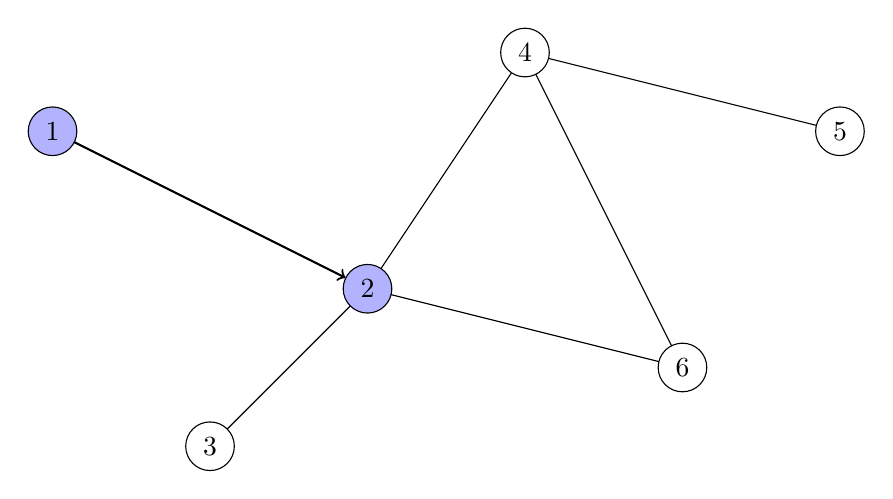
\begin{tikzpicture}
        \draw[thick,->] (0,7) -- (3.72,5.14);
        \draw (4,5) -- (2,3);
        \draw (4,5) -- (6,8);
        \draw (4,5) -- (8,4);
        \draw (6,8) -- (10,7);
        \draw (6,8) -- (8,4);

        \node[circle, draw, fill=blue!30] at (0, 7) {1};
        \node[circle, draw, fill=blue!30] at (4, 5) {2};
        \node[circle, draw, fill=white] at (2, 3) {3};
        \node[circle, draw, fill=white] at (6, 8) {4};
        \node[circle, draw, fill=white] at (10, 7) {5};
        \node[circle, draw, fill=white] at (8, 4) {6};

    \end{tikzpicture}

\end{frame}

\begin{frame}[fragile]{Visualização da identificação de ciclos}

    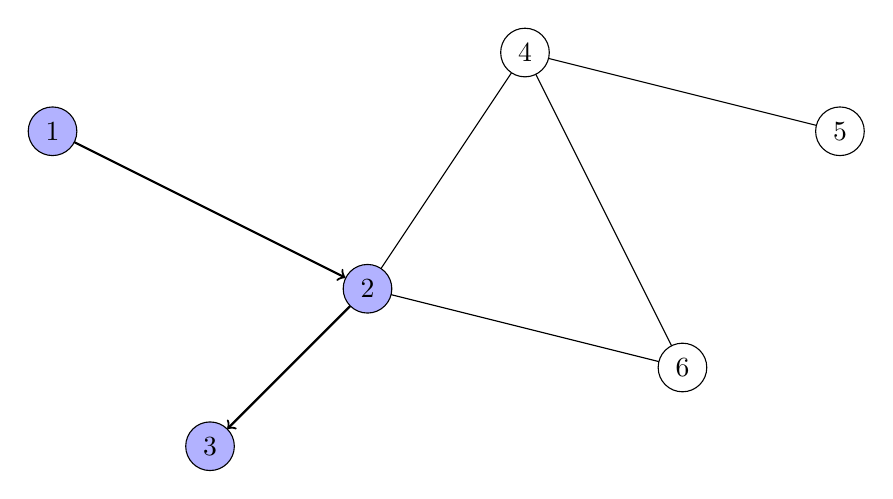
\begin{tikzpicture}
        \draw[thick,->] (0,7) -- (3.72,5.14);
        \draw[thick,->] (4,5) -- (2.22,3.22);
        \draw (4,5) -- (6,8);
        \draw (4,5) -- (8,4);
        \draw (6,8) -- (10,7);
        \draw (6,8) -- (8,4);

        \node[circle, draw, fill=blue!30] at (0, 7) {1};
        \node[circle, draw, fill=blue!30] at (4, 5) {2};
        \node[circle, draw, fill=blue!30] at (2, 3) {3};
        \node[circle, draw, fill=white] at (6, 8) {4};
        \node[circle, draw, fill=white] at (10, 7) {5};
        \node[circle, draw, fill=white] at (8, 4) {6};

    \end{tikzpicture}

\end{frame}

\begin{frame}[fragile]{Visualização da identificação de ciclos}

    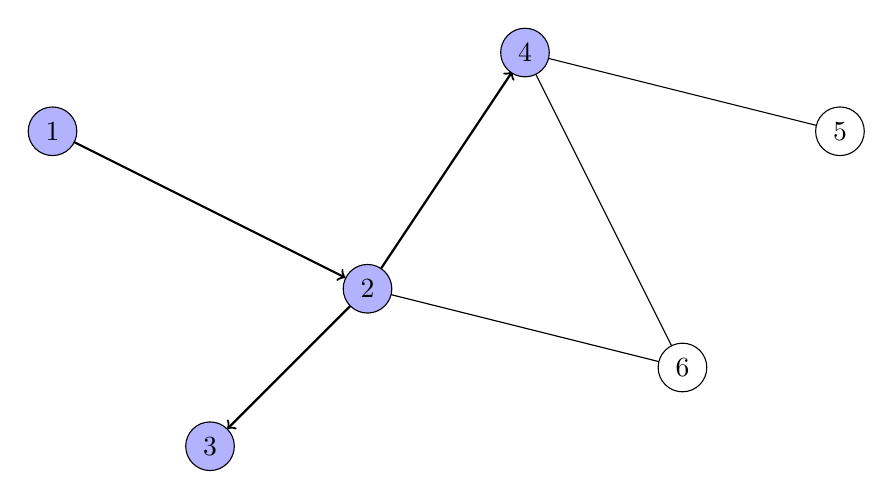
\begin{tikzpicture}
        \draw[thick,->] (0,7) -- (3.72,5.14);
        \draw[thick,->] (4,5) -- (2.22,3.22);
        \draw[thick,->] (4,5) -- (5.84,7.76);
        \draw (4,5) -- (8,4);
        \draw (6,8) -- (10,7);
        \draw (6,8) -- (8,4);

        \node[circle, draw, fill=blue!30] at (0, 7) {1};
        \node[circle, draw, fill=blue!30] at (4, 5) {2};
        \node[circle, draw, fill=blue!30] at (2, 3) {3};
        \node[circle, draw, fill=blue!30] at (6, 8) {4};
        \node[circle, draw, fill=white] at (10, 7) {5};
        \node[circle, draw, fill=white] at (8, 4) {6};

    \end{tikzpicture}

\end{frame}

\begin{frame}[fragile]{Visualização da identificação de ciclos}

    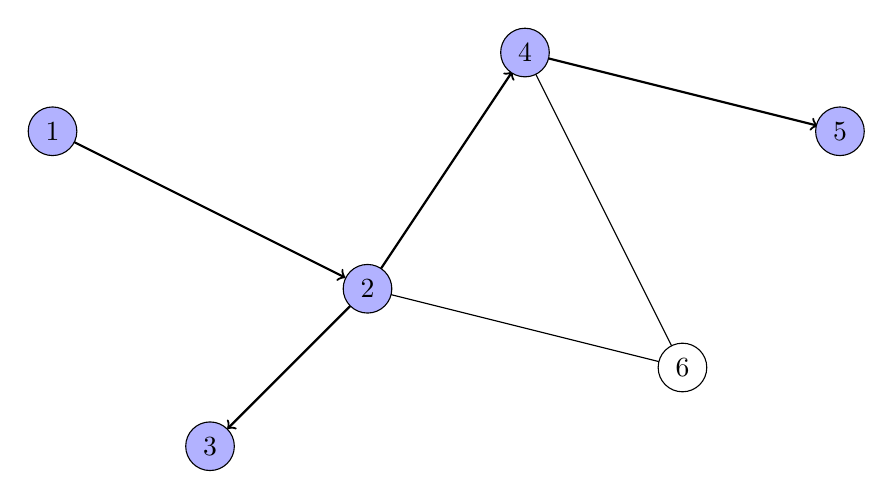
\begin{tikzpicture}
        \draw[thick,->] (0,7) -- (3.72,5.14);
        \draw[thick,->] (4,5) -- (2.22,3.22);
        \draw[thick,->] (4,5) -- (5.84,7.76);
        \draw[thick,->] (6,8) -- (9.72,7.07);
        \draw (6,8) -- (8,4);
        \draw (4,5) -- (8,4);

        \node[circle, draw, fill=blue!30] at (0, 7) {1};
        \node[circle, draw, fill=blue!30] at (4, 5) {2};
        \node[circle, draw, fill=blue!30] at (2, 3) {3};
        \node[circle, draw, fill=blue!30] at (6, 8) {4};
        \node[circle, draw, fill=blue!30] at (10, 7) {5};
        \node[circle, draw, fill=white] at (8, 4) {6};

    \end{tikzpicture}

\end{frame}

\begin{frame}[fragile]{Visualização da identificação de ciclos}

    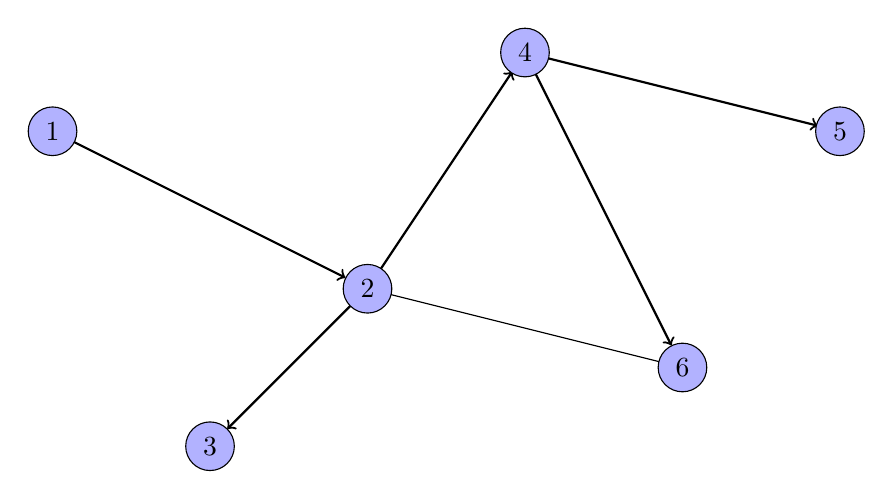
\begin{tikzpicture}
        \draw[thick,->] (0,7) -- (3.72,5.14);
        \draw[thick,->] (4,5) -- (2.22,3.22);
        \draw[thick,->] (4,5) -- (5.84,7.76);
        \draw[thick,->] (6,8) -- (9.72,7.07);
        \draw[thick,->] (6,8) -- (7.86,4.28);
        \draw (4,5) -- (8,4);

        \node[circle, draw, fill=blue!30] at (0, 7) {1};
        \node[circle, draw, fill=blue!30] at (4, 5) {2};
        \node[circle, draw, fill=blue!30] at (2, 3) {3};
        \node[circle, draw, fill=blue!30] at (6, 8) {4};
        \node[circle, draw, fill=blue!30] at (10, 7) {5};
        \node[circle, draw, fill=blue!30] at (8, 4) {6};

    \end{tikzpicture}

\end{frame}

\begin{frame}[fragile]{Visualização da identificação de ciclos}

    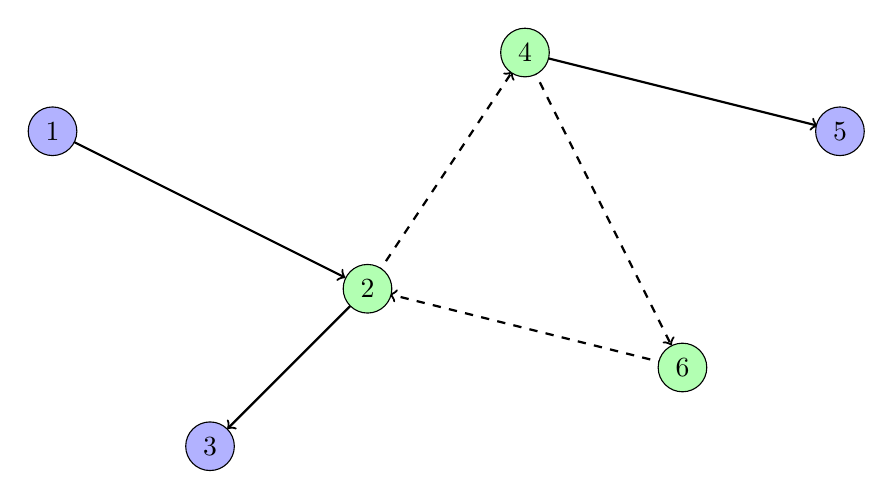
\begin{tikzpicture}
        \draw[thick,->] (0,7) -- (3.72,5.14);
        \draw[thick,->] (4,5) -- (2.22,3.22);
        \draw[thick,->,dashed] (4,5) -- (5.84,7.76);
        \draw[thick,->] (6,8) -- (9.72,7.07);
        \draw[thick,->,dashed] (6,8) -- (7.86,4.28);
        \draw[thick,->,dashed] (8,4) -- (4.28,4.93);

        \node[circle, draw, fill=blue!30] at (0, 7) {1};
        \node[circle, draw, fill=green!30] at (4, 5) {2};
        \node[circle, draw, fill=blue!30] at (2, 3) {3};
        \node[circle, draw, fill=green!30] at (6, 8) {4};
        \node[circle, draw, fill=blue!30] at (10, 7) {5};
        \node[circle, draw, fill=green!30] at (8, 4) {6};

    \end{tikzpicture}

\end{frame}

\begin{frame}[fragile]{Exemplo de detecção de ciclo}
    \inputsnippet{c++}{1}{18}{check.cpp}
\end{frame}

\begin{frame}[fragile]{Exemplo de detecção de ciclo}
    \inputsnippet{c++}{19}{39}{check.cpp}
\end{frame}

\begin{frame}[fragile]{Exemplo de detecção de ciclo}
    \inputsnippet{c++}{40}{60}{check.cpp}
\end{frame}

\begin{frame}[fragile]{Outro exemplo de detecção de ciclo}
    \inputsnippet{c++}{1}{21}{check2.cpp}
\end{frame}

\begin{frame}[fragile]{Outro exemplo de detecção de ciclo}
    \inputsnippet{c++}{23}{43}{check2.cpp}
\end{frame}

\begin{frame}[fragile]{Outro exemplo de detecção de ciclo}
    \inputsnippet{c++}{45}{65}{check2.cpp}
\end{frame}
